\documentclass[a4paper,12pt]{report}    % Document Class
% % % % % % % % % % % % % % % % % % % % % % % % % % % % % % % % %
% % % % PACKAGES
% % % % % % % % % % % % % % % % % % % % % % % % % % % % % % % % %
\linespread{1.5}                    % For line spacing
\usepackage{amssymb}                % For AMS symbol
\usepackage{amsmath}                % This is useful for the matrix 
\usepackage{verbatim}               % For comments in paragraph
\usepackage{graphicx}               % For imbeding graph
\usepackage{color}                  % Color for the text
\usepackage{makeidx}
\usepackage{url}
%\usepackage{apacite}
\usepackage{sectsty}
\chapterfont{\centering}



% % % % % % % % % % % % % % % % % % % % % % %
% % % % FOR ADJUSTMENT OF PAGES
% % % % % % % % % % % % % % % % % % % % % % %
\usepackage[top=2cm, bottom=2cm, left=3cm, right=2cm]{geometry}

% % % % % % % % % % % % % % % % % % % % % % % %
% % % % FOR SHORTCUT USE
% % % % % % % % % % % % % % % % % % % % % % % %
\newtheorem{df}{Definition} % For definition
\newtheorem{exm}{Example}   % For Example
\newtheorem{exe}{Exercise}  % For Exercise
\newtheorem{prob}{Problem}  % For Problem
\newtheorem{task}{TASK}     % For Task
\newtheorem{thm}{Theorem}   % For Theorem
% % % % % % % % % % % % % % % % % % % % % % % % %
\renewcommand{\chaptername}{CHAPTER}
\renewcommand{\contentsname}{\centering CONTENTS}
\renewcommand{\listfigurename}{\centering LIST OF FIGURES}
\renewcommand{\listtablename}{\centering LIST OF TABLES}

%%%%%%%%%%%%%%%%%%%%%%%%%%%%%%%%%%%%%%%%%%%%%%%%%%%%%%%
\pagestyle{plain}
%==================================================================
\begin{document}
% % % % % % % % % % % % %
\pagenumbering{roman}
%===================================================================
%   Begin your document hereafter
%=====================================================================



{\large
\begin{center}
{{\bf{\color{red}SEE-MATH : A Math Visualization Website}}}\\
\end{center}


\vspace{0.8cm}

{\normalsize
\begin{center}
A THIRD YEAR PROJECT REPORT\\

\vspace{0.5cm}
SUBMITTED IN PARTIAL FULFILLMENT OF THE REQUIREMENTS FOR\\
THE DEGREE OF B.Sc. IN COMPUTATIONAL MATHEMATICS\\

\vspace{1.0cm}

BY
\end{center}
\begin{center}
\begin{itemize}
\begin{center}

\item[1.] Mukesh Tiwari (026615-19)
\item[2.] Bishesh Kafle (026600-19)
\item[3.] Priyanka Panta (026605-19)
\item[4.] Prajanya Parakram Shrestha (026614-19)
\end{center}
\end{itemize}

\end{center}


\vspace{1.0cm}

\begin{figure}[htpb]
\centering

\includegraphics[height=4.5cm,width=4.5cm]{photos/kulogo.jpg}
\end{figure}


\vspace{2cm}
{\normalsize
\begin{center}
%DEPARTMENT OF NATURAL SCIENCES (MATHEMATICS)\\
SCHOOL OF SCIENCE\\
KATHMANDU UNIVERSITY\\
DHULIKHEL, NEPAL\\
\end{center}
}

\begin{center}
	{\color{red} November 2022}
\end{center}

}
}

%\underbrace{}
\thispagestyle{empty}	% No numbering in this page

%===================================================================
%\newpage
%\input{Dedication}

%\newpage
%\input{Student_declaration}

\newpage



%\addcontentsline{toc}{chapter}{\bf Certification}
\addcontentsline{toc}{chapter}{\bf CERTIFICATION}

\begin{center}
	{\Large{\bf{ CERTIFICATION}}}
\end{center}


\noindent
This project entitled "SEE-Math : A Math Visualization Website" is carried out  under my supervision for the specified entire period satisfactorily, and is hereby certified as a work done by following students
\begin{itemize}
\item[1.] Prajanya Parakram Shrestha (Exam Roll No.)
\item[2.] Bishesh Kafle (Exam Roll No.)
\item[3.] Priyanka Panta (Exam Roll No.)
\item[4.] Mukesh Tiwari (Exam Roll No.)
\end{itemize}
 in partial fulfillment of the requirements for the degree of B.Sc. in Computational Mathematics, Department of Mathematics, Kathmandu University, Dhulikhel, Nepal.

\vspace{2.0cm}

\noindent
--------------------------\\
{\bf Dr. Samir Shrestha}\\
Associate Professor \\
Department of Mathematics,\\
School of Science, Kathmandu University,\\
Dhulikhel, Kavre, Nepal\\
Date:\today

\vspace{2cm}

\noindent
{\bf APPROVED BY:}\\
I hereby declare that the candidate qualifies to submit this  report of the Computer Project (Comp-311) to the Department of Mathematics. 



\vspace{2cm}

\noindent
-----------------------------\\
Head of the Department\\
Department of Mathematics\\
School of Science\\
Kathmandu University\\
Date:\today
  


\newpage



%\addcontentsline{toc}{chapter}{\bf Acknowledgements}
\addcontentsline{toc}{chapter}{\bf ACKNOWLEDGEMENTS}
%{\Large{\bf{ACKNOWLEDGMENTS}}}\\

\begin{center}
	{\Large{\bf{ACKNOWLEDGMENTS}}}\\
\end{center}

\noindent

This project has been carried out under the supervision of Dr. Samir Shrestha from the Department of Mathematics and Mr. Amrit Dahal from the Department of Computer Science and Engineering. We would like to express our sincere gratitude towards our supervisors for their excellent supervision, guidance, and suggestion for accomplishing this work and to the entire faculty of the Department of Mathematics for encouraging, supporting, and providing this opportunity to learn and explore.\\

\noindent
We are indebted to our friends for motivating us throughout. \\

\noindent
Lastly, we would like to thank everyone who helped us directly and indirectly during the completion of our project work.





\newpage



%\addcontentsline{toc}{chapter}{\bf Abstract}
\addcontentsline{toc}{chapter}{\bf ABSTRACT}

\begin{center}
	{\Large{\bf{ABSTRACT}}}\\
\end{center}

\noindent
This project aims to implement the numerical method algorithms, namely Bisection and Newton-Rhapson along with their step-wise visualization in a web page. This will be beneficial to students and teachers in classrooms for explanation and intuition regarding these topics and also aid self-exploration into these materials. The demonstrations are fully client side and written in JS using popular and powerful libraries like JSXgraph.



% ===================================================================

\tableofcontents


\listoffigures
%\addcontentsline{toc}{chapter}{List of Figures}
\addcontentsline{toc}{chapter}{LIST OF FIGURES}

\listoftables
%\addcontentsline{toc}{chapter}{List of Tables}
\addcontentsline{toc}{chapter}{LIST OF TABLES}

\newpage




%\addcontentsline{toc}{chapter}{\bf List of Symbols}
\addcontentsline{toc}{chapter}{\bf LIST OF SYMBOLS}

\begin{center}
	{\LARGE{\bf{LIST OF SYMBOLS}}}\\
\end{center}


Your parameters here.

% ====================================================================
\newpage
\pagenumbering{arabic}

%\addcontentsline{toc}{chapter}{\bf cHA}

%\begin{center}
%	{\Large{\bf{CHAPTER 1}}}\\
%\end{center}

%\addcontentsline{toc}{chapter}{\bf Acknowledgements}
%\addcontentsline{toc}{chapter}{\bf ACKNOWLEDGEMENTS}

%\begin{center}
%	{\Large{\bf{CHAPTER 1}}}\\
%\end{center}

\chapter{Introduction}

\section{{\bf{Background}}}








\section{{\bf{Objectives}}}
{\bf\color{black}
\begin{enumerate}
 \item
 \item 
 \item 
 \item 
\end{enumerate}
}

\section{\bf Motivation And Sigificance}
{\bf\color{red}In this section, the author(s) shall discuss the relevance and the underlying problems that may rise to the need to do this project/work.}
\begin{table}[htpb]
\caption{Name and Notation.}
\begin{center}
\begin{tabular}{|c|c|c|}\hline
Category & Intuitive meaning & Typical element \\ \hline
                                                    \hline
$\mathit{Nml}$ & numerals & $N$ \\ \hline
$\mathit{UnOps}$ & unary operators & $\alpha$ \\ \hline
$\mathit{BinOps}$ & binary operators & $\omega$ \\ \hline
$\mathit{Ide}$ & identifiers & $I$ \\ \hline
$\mathit{Exp}$ & expressions & $E$ \\ \hline
$\mathit{Cmd}$ & commands & $C$ \\ \hline
\end{tabular}
\end{center}
\end{table}



%\newpage
%
\chapter{Related Works}
\noindent

See-math is website for solving and visualizing various mathematical problems. The approach of solving problems is table based and graph based. Numerous works related to visualizing mathematical problems have been previously done, some of them being codesansaar.com, atozmath.com, keisan.casio.com, planetcalc.com and many more. Most of the mentioned websites solve the problems and display output table-based without graphical representations but some websites such as planetcalc.com have improved by taking into consideration previous works and adding new aproaches such as graphical representaions along with table based ones but yet have not made visualization possible for all mathematical problems. \\

\noindent
The main contribution of our work to this problem is the implementation of graph based visualization along with table based outputs. The impact of our approach that adresses these existing limitation is going to help on better understanding of various mathematical problems.


\newpage

\chapter{Design And Implementation}

The first step in this project was to choose a framework and type of website we wanted to build. We had two options : 
\begin{itemize}
	\item Static Website
	\item Dynamic Website
\end{itemize}
Dynamic Website provided us with great flexibility in the choice of programming language. It was much easier to build using existing libraries and tools. However, It was costly to deploy because an active server running the scripts on the back end as per the requests is needed. The programs to implement the various algorithms of numerical methods are not too complex and require no database.

On the other hand, static sites can be run on the client side but the lack of libraries specific to mathematical visualization and functions meant that we had to code a lot of it by ourselves. They are however free to deploy and serve.

We went with the static option and decided to use Jekyll, which is a static website generator. It utilizes markdown along with HTML and CSS to easily generate websites that are blog-like. The following figure show this.

\begin{figure}[h!]
	\centering
	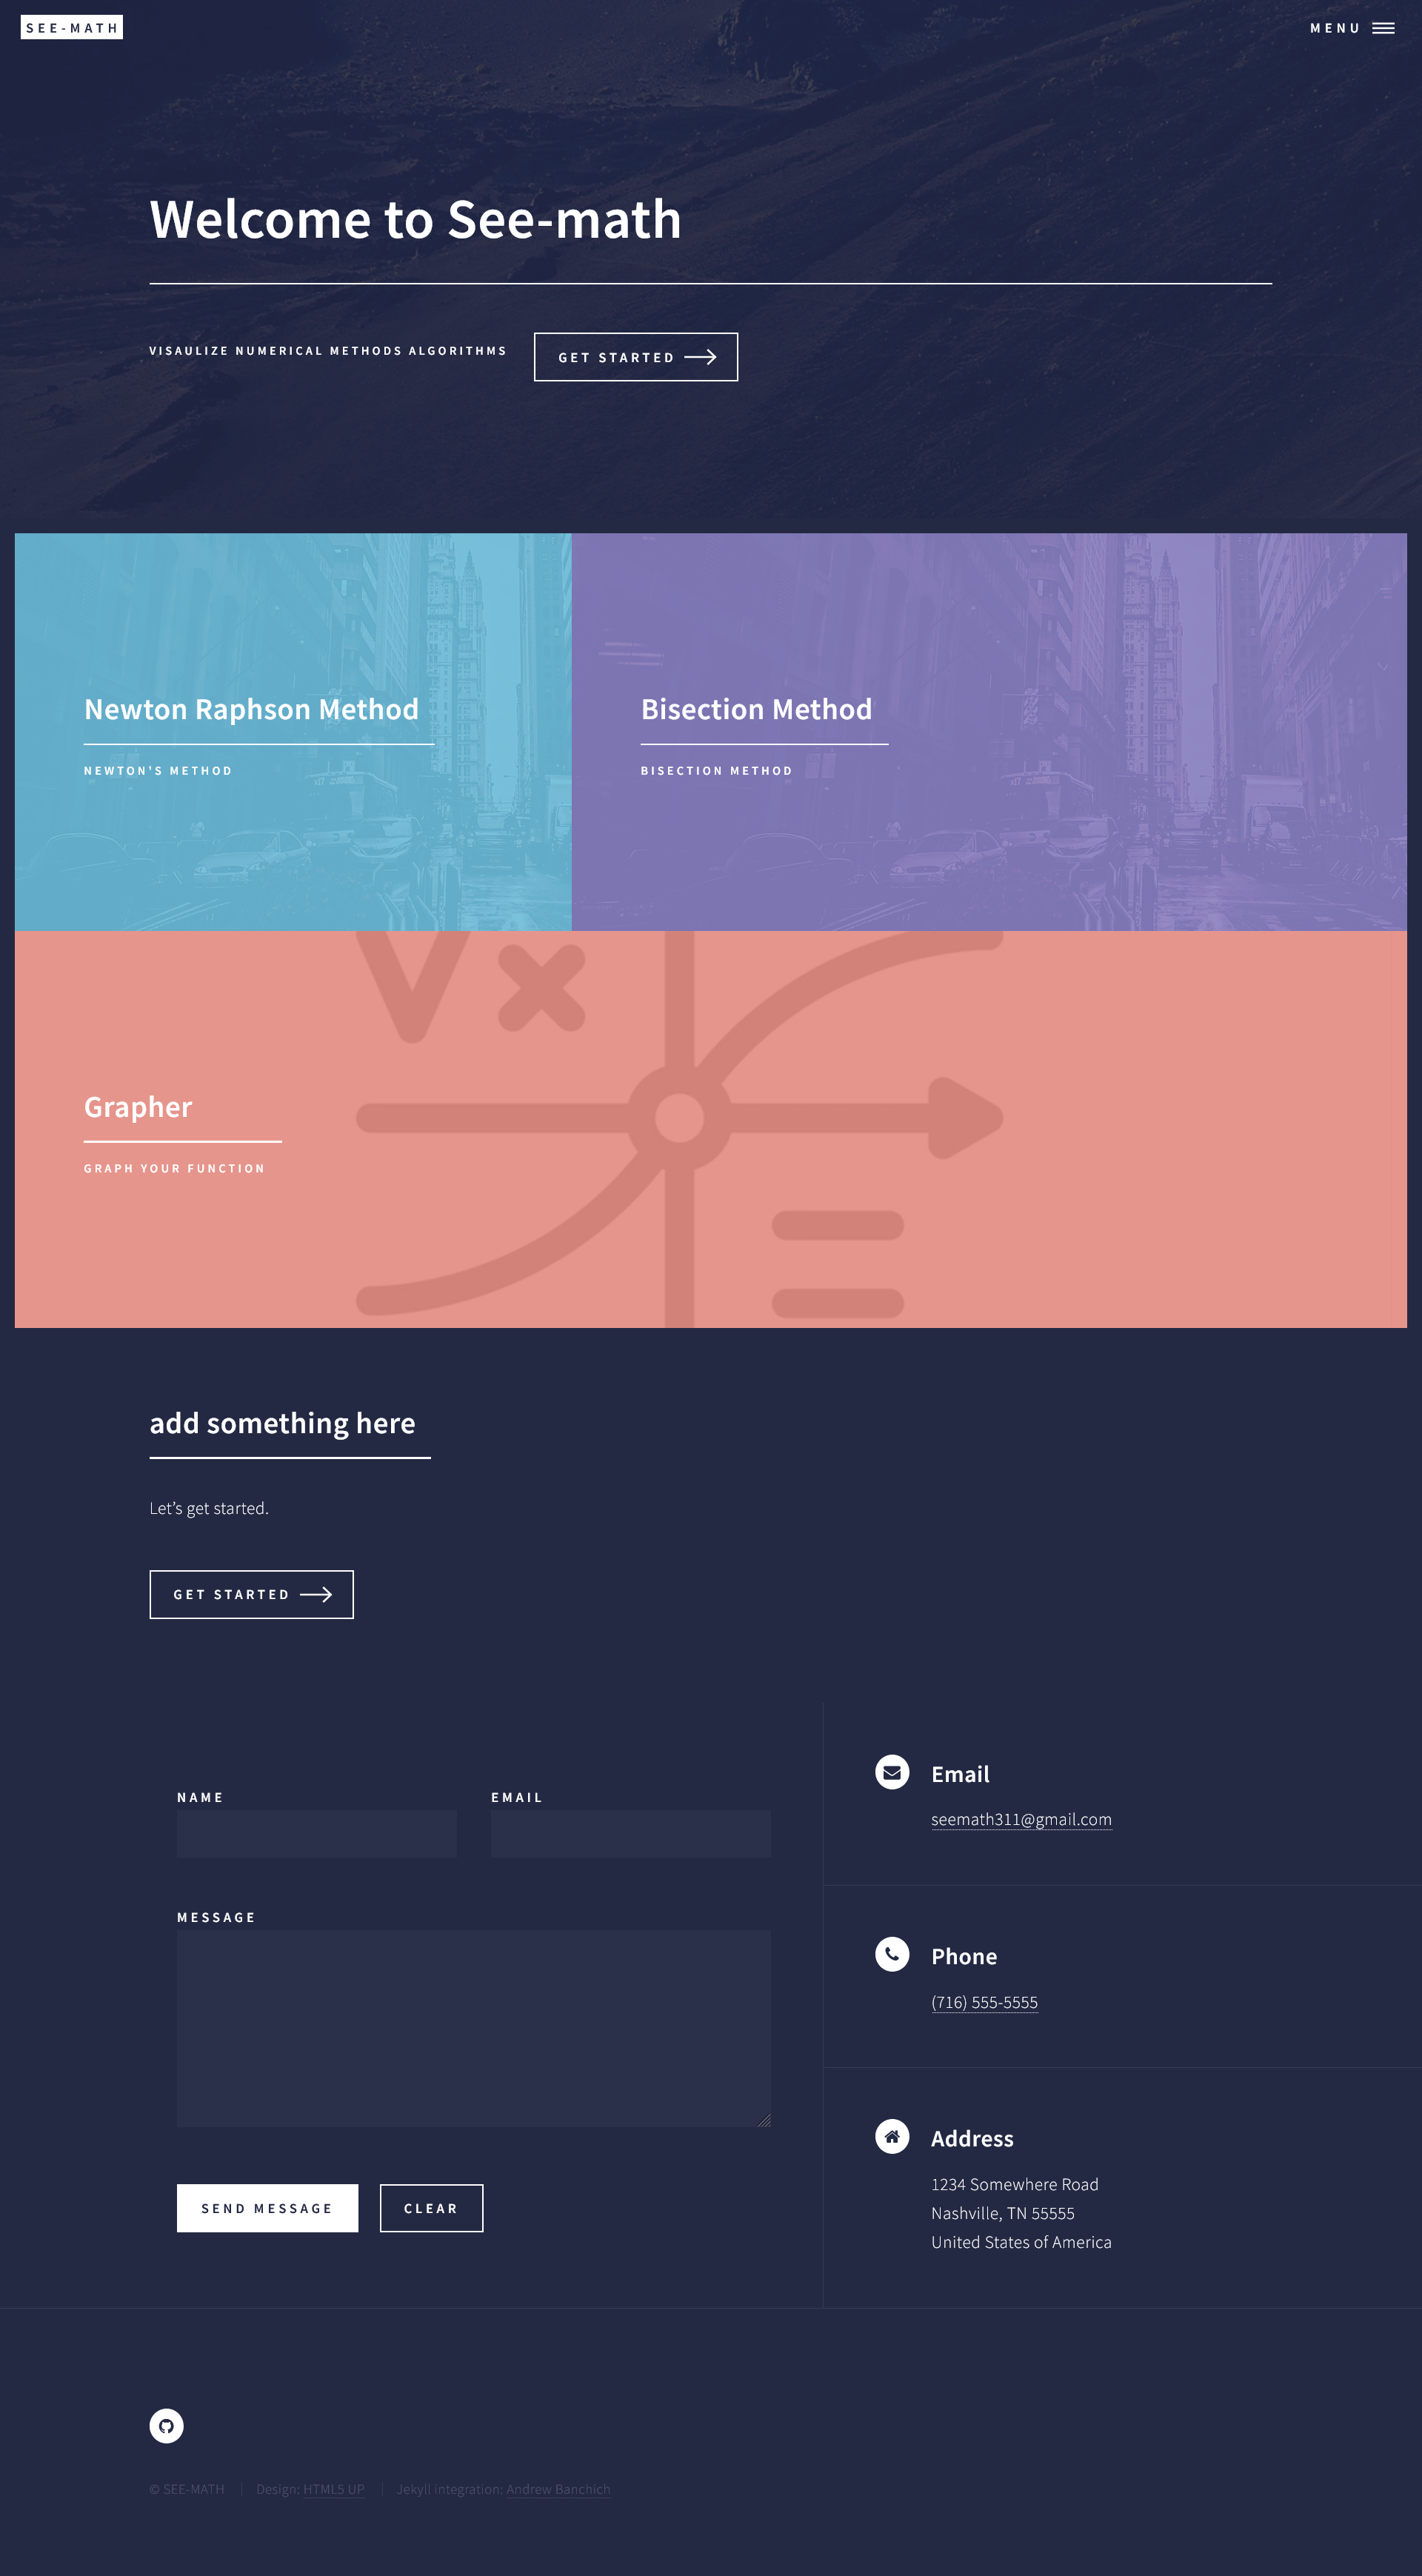
\includegraphics[width=0.8\linewidth]{seemath1}
	\caption{UI layout of website}
\end{figure}

\pagebreak
The next step was to design the method for getting user inputs, which are mathematical formulas in our case, and converting them to functions. We also needed to get a way to plot them and display the output. We utilized various libraries like 'math.js', 'mathjax.js', and 'plotly.js' to get the desired result.

\begin{figure}[h!]
	\centering
	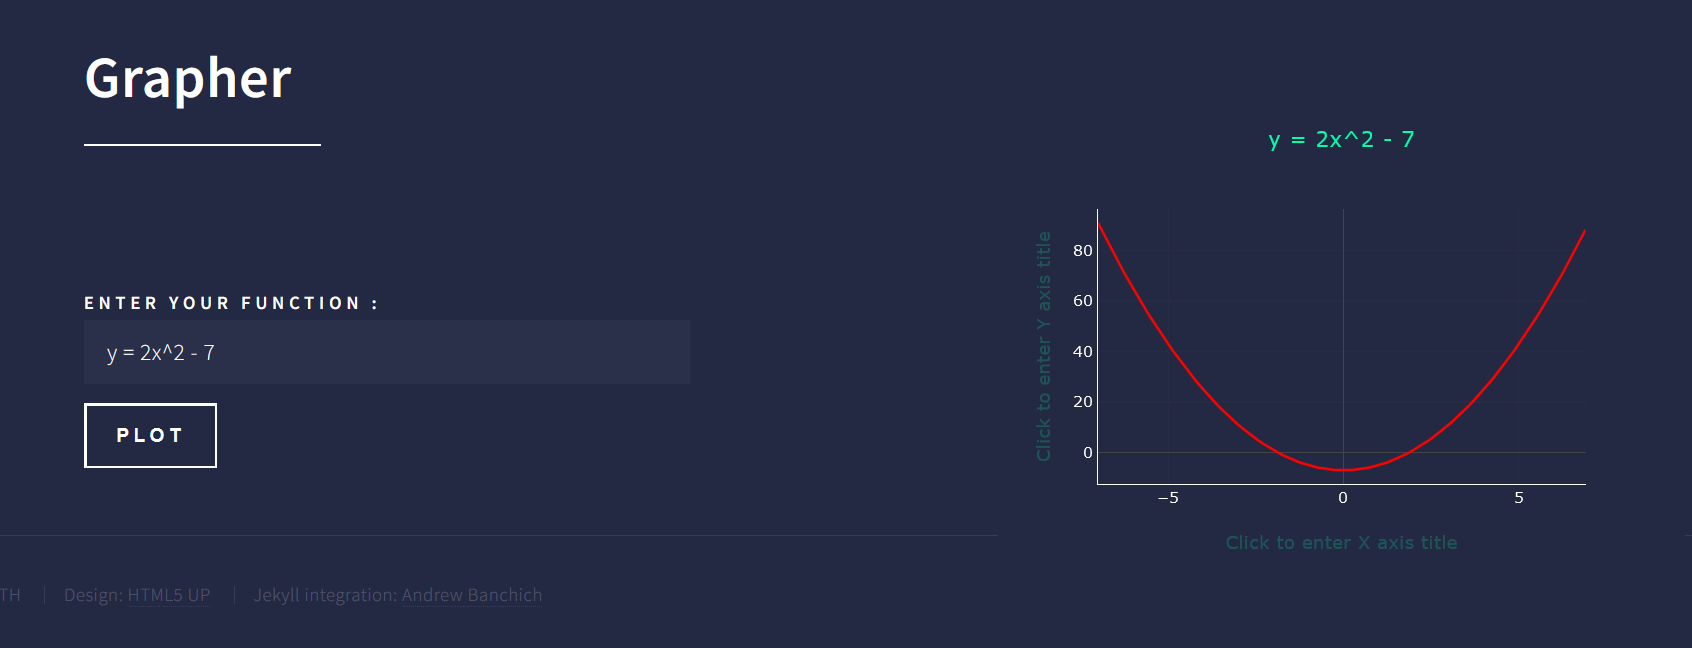
\includegraphics[width=0.89\linewidth]{seemath3}
	\caption{Input and Graphing Features}
\end{figure}

However, for getting step-wise solutions and visualizations associated with each iteration of algorithms like Bisection or Newton-Rhapson, we need a canvas-like library to be able to draw and remove geometrical objects. After extensive research, we found that 'JSXgraph' fitted the bill. we then began with implementing the algorithms and then the steps to visualize them in JS.

\begin{figure}[h!]
	\centering
	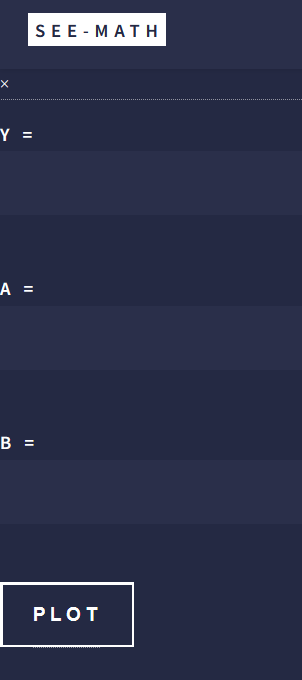
\includegraphics[width=0.24\linewidth]{seemath4}
	\caption{User Input for Bisection}
\end{figure}

\pagebreak
The graphs for both the methods are generated by using plot button. the next and animate button show the iterations with animation. Each graph can be panned, zoomed and interacted with. 
There are no zoom and pan feature in the JSXgraph library. Thus, we had to look at other methods. We utilized the fact that we could change the boundary box of the graph and changed it in a slow and controlled way to slowly transition from one state to another.
\begin{figure}[h!]
	\centering
	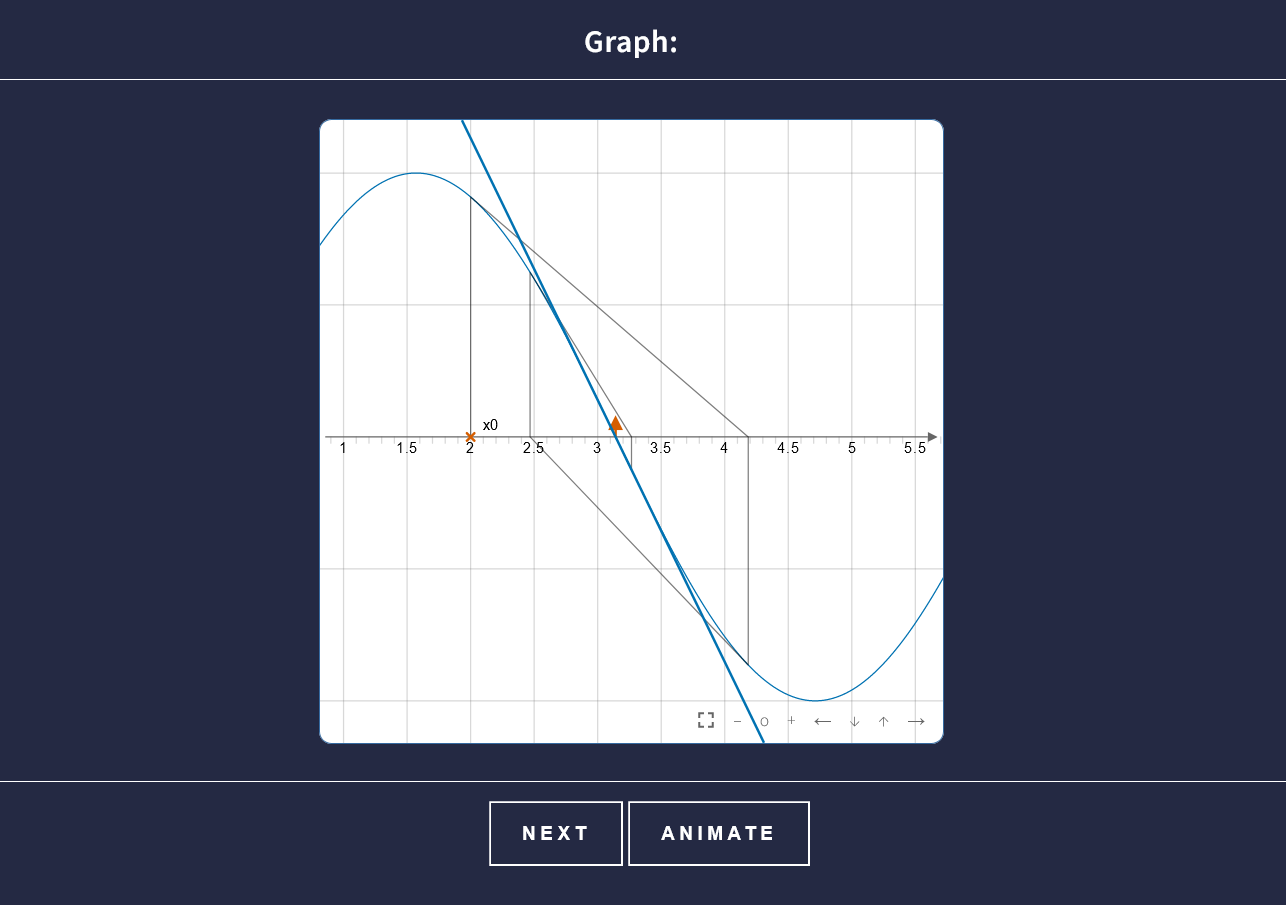
\includegraphics[width=0.89\linewidth]{seemath6}
	\caption{Newton Rhapson Method}
\end{figure}

\begin{figure}[h!]
\centering
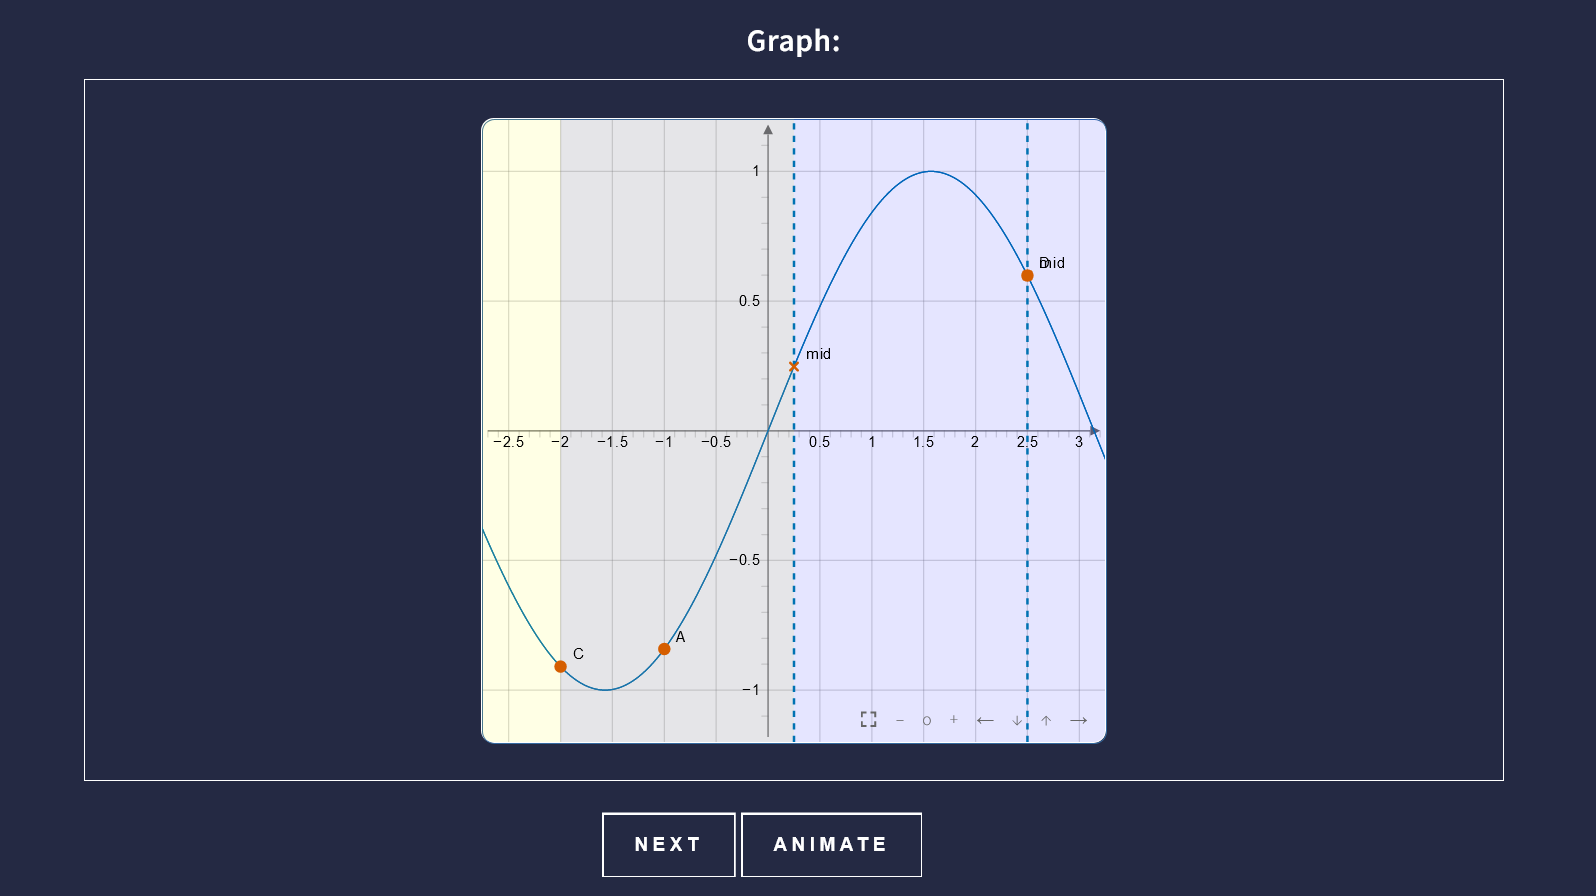
\includegraphics[width=0.89\linewidth]{seemath7}
\caption{Bisection Method}
\end{figure}

\pagebreak
To make getting feedback and suggestions easier, we added a contact form. Since there is no dynamic elements in our website or a central server to receive the feedback and process it. We utilized a service known as 'Formspree'\cite{form} to get emails containing the feedback.

\begin{figure}[h!]
	\centering
	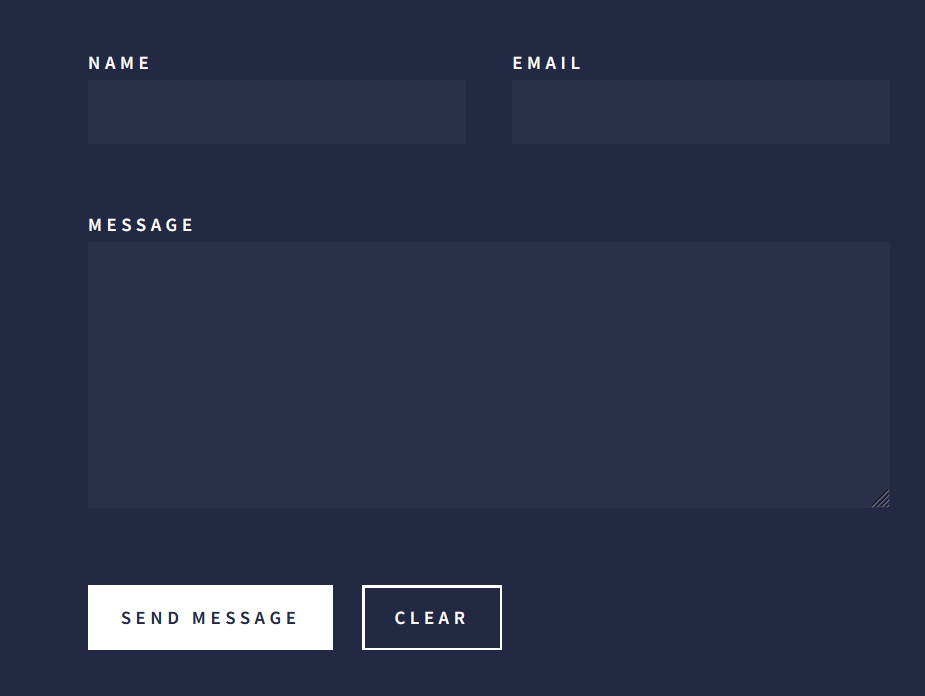
\includegraphics[width=0.5\linewidth]{seemath5}
	\caption{Feedback Form}
\end{figure}


\newpage

\chapter{System Requirement Specification}

\section{{\bf{Software Specification}}}


\subsection{{\bf{Front-End Tools}}}


\subsection{{\bf{Back-End Tools}}}

\subsection{{\bf{Utility Tools}}}


\section{{\bf{Hardware Specification}}}
\newpage
\chapter{Discussion On The Achievements}

This project has been a topic that was completely new for all of us team members. With interests on learning web development, knowing how they operate and with a motive to construct a tool, that not only supports us as a learners base, but has the ability to be used for practical learning and making concepts plain and understandable. The following work has been achieved as a result of this project:
\begin{itemize}
	\item Gained a deep understanding of web frameworks, communication with the server and user-interaction.
	\item Built proficiency in scripting for websites as well as developed a hint for web design.
	\item A completely working graphing function, that plots the user defined curves has been integrated.
	\item Root finding through bisection method and Newton-Raphson method has been successfully implemented.
	\item Implemented the functionality to message the developers for reviews and complaints.
\end{itemize}


\section{{\bf{Features}}}

See-math promises to be a great visualization tool for various numerical method algorithms as well as the construction of finite automata machines. Till date, the following features have been integrated on our website:
\begin{itemize}
	\item A message form for interaction.
	\item Grapher : Plots the given function.
	\item Bisection Method
	\item Newton-Raphson Method
\end{itemize}

\section{{\bf{Limitations}}}

See-math is a website meant for visualizing mathematcal problems and gaining better understanding of the problem. The goal of the website is to solve and visualize as much mathematical problems as possible but current only some of the problems reated to numerical methods such as bisection methon and newton raphson method can be fully calculated and visualized.

\section{{\bf{Future Enhancements}}}

The current see-math lacks in comaprisoin to the ideal visualization website meant to solve numerous mathematical problems. Various methods are yet to be added and many enhancements are yet to be made and in the near future various features and new method will slowly but surely be included.

\newpage
\chapter{Conclusion And Recommendation}

\section{{\bf{Limitations}}}

\section{{\bf{Future Enhancements}}}


\newpage


%=====================================================================
% For Reference settings
%%%%%%%%%%%%%%%%%%%%%%%%%%%%%%%%%%%%%%%%%%%%%%%%%%%%%%%%%%%%%%%%%%%%%
\renewcommand{\bibname}{\centering REFERENCES}
\bibliographystyle{amsplain}

\bibliography{bibtex_database/myrefs} % data base
%===================================================================
\end{document}
